\chapter{Quantum-mechanical harmonic oscillator}

The previous chapter introduced the phenomenological description of shot noise and ASE to calculate SNR in various optical measurements. Quantum optics tells you the physics behind these noise sources and provides ways to manipulate them.

In quantum optics, the physics of harmonic oscillators play a crucial role because electromagnetic field is decomposed into the collection of time-frequency modes, spatial modes, and polarizations, and each mode is assumed as a quantum-mechanical harmonic oscillator. 

This chapter will introduce the quantum-mechanical harmonic oscillators. If you are familiar with the basics of quantum mechanics, you can skip this chapter.

\section{Schr\"odinger equation for a harmonic oscillator}
\subsection{Classical harmonic oscillators}

Let's discuss the motion of a one-dimensional mass-spring system without friction with a mass of $m$ and a spring constant of $k$. The equation of motion of the position $X(t)$ of the mass as a function of time is given by
\begin{equation}
  m\frac{d^2X}{dt^2}+kX = 0.
\end{equation}
The solution is given by
\begin{equation}
  X(t) = \frac 1 2 A \exp (-i\omega t) + c.c. = \mathrm{Re}[A\exp(-i\omega t)]
 \label{eq:solution_of_classical_harmonic_oscillator}
\end{equation}
where $A$ is a complex number, $\omega = \sqrt{k/m}$, and $c.c.$ stands for the complex conjugate. The momentum $P = m (dX/dt)$ is given by
\begin{equation}
  P(t) = \frac {-im\omega}{2}A\exp(-i\omega t)+c.c. = m\omega\mathrm {Im}[A\exp(-i\omega t)].
  \label{eq:solution_of_classical_harmonic_oscillator_momentum}
\end{equation}
Eq. (\ref{eq:solution_of_classical_harmonic_oscillator}) and Eq. (\ref{eq:solution_of_classical_harmonic_oscillator_momentum}) show that $X(t)$ and $P(t)$ oscillate while keeping a phase difference of 90 degree.

The sum of potential energy and kinetic energy is given by
\begin{equation}
  E = \frac{1}{2}kX^2 + \frac{m}{2}\left(\frac{dX}{dt} \right)^2 = \frac{1}{2}kX^2 + \frac{P^2}{2m},
  \label{eq:total_energy}
\end{equation}
where we introduced the momentum $P = m(dX/dt)$. Substituting Eq. (\ref{eq:solution_of_classical_harmonic_oscillator}) to Eq. (\ref{eq:total_energy}), we obtain
\begin{equation}
  E= \frac{1}{2}k(\mathrm{Re} [A\exp(-i\omega t)])^2 + \frac{m\omega^2}{2} (\mathrm{Im} [A\exp(-i\omega t)])^2 = \frac{1}{2}k|A|^2.
\end{equation}
In this way, we can see that the total energy is kept constant.
The above results are general in harmonic oscillators: each oscillator has two degrees of freedom, and they oscillate with 90-degree phase difference. To further generalize the result, we introduce the normalized position $x$ and the normalized momentum $p$ such that the potential energy is given by $\hbar \omega x^2$ and the kinetic energy is given by $\hbar \omega p^2$, i.e., Eq. (\ref{eq:total_energy}) becomes
\begin{equation}
  E = \hbar \omega (x^2 + p^2).
\end{equation}
This is made possible by defining $x$ and $p$ as
\begin{equation}
  x = \sqrt \frac{k}{2\hbar\omega} X,
  \label{eq:normalized_position}
\end{equation}
\begin{equation}
  p = \frac{1}{\sqrt{2m\hbar \omega}}P,
  \label{eq:normalized_momentum}
\end{equation}
respectively. Since $\hbar \omega$ is the energy unit of quantum harmonic oscillators, such normalization can simplify the notation and therefore they are often used. We also introduce the normalized complex amplitude
\begin{equation}
  a = \sqrt{\frac{k}{2\hbar \omega}}A
\end{equation}
so that the time evolution of $x$ and $p$ are given by
\begin{equation}
  x(t) = \mathrm{Re}[a \exp(-i\omega t)],
\end{equation}
\begin{equation}
  p(t) = \mathrm{Im}[a \exp(-i\omega t)],
\end{equation}
respectively. Also, we can define $a(t) = a\exp(-i\omega t)$, which satisfies
\begin{equation}
  a(t) = x(t) + ip(t).
  \label{eq:normalized_complex_amplitude}
\end{equation}
You can see that $x(t)$ and $p(t)$ in the $x$-$p$ plane, which is called phase space, form a circular trajectory rotating at a frequency of $\omega$, as shown in Fig. {\ref{fig:classical_phase_space}}(a). This is a very general property of classical harmonic oscillator. 

In the later chapters, you will see that in quantum harmonic oscillator $x(t)$ and $p(t)$ have certain fluctuation or uncertainty, as conceptually illustrated in Fig. {\ref{fig:classical_phase_space}}(b). This results in the shot noise and optical amplifier noise.

\begin{figure}
  \centering
  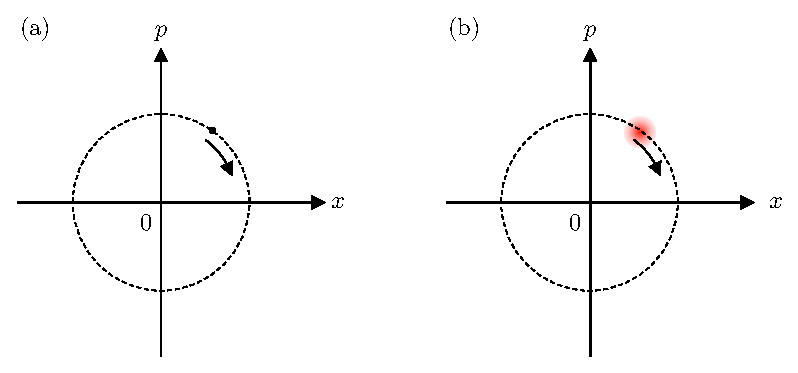
\includegraphics[width=9cm]{fig/3-1_phase_space.eps} 
  \caption{Evolution of position $x(t)$ and momentum $p(t)$ in the phase space. (a) Classical harmonic oscillator. (b) Quantum harmonic oscillator. }
  \label{fig:classical_phase_space}
\end{figure}


\subsection{Wavefunctions and Schr\"odinger equation}
To introduce quantum-mechanical harmonic oscillators, we start from de Broglie's relation, which assumes a complex wavefunction with a temporal angular frequency $\Omega$ and spatial angular frequency $K$, which are related to the energy and the momentum by
\begin{equation}
  E = \hbar \Omega,
\end{equation}
\begin{equation}
  P = \hbar K,
\end{equation}
respectively. If we consider an exemplary wavefunction denoted as $\Phi(X, t)= \exp[i(KX-\Omega t)]$, we get 
\begin{equation}
 i\hbar\frac{\partial\Phi}{\partial t} = \hbar\Omega \Phi = E\Phi,
\end{equation}
\begin{equation}
-i\hbar \frac {\partial \Phi}{\partial X} = \hbar K\Phi = P\Phi.
\end{equation}
Suggested by the above equations, we define the following operators:
\begin{equation}
	\hat E \equiv i\hbar \frac{\partial}{\partial t}, 
 \label{eq:energy_operator}
\end{equation}
\begin{equation}
  \hat P \equiv -i\hbar \frac{\partial}{\partial X},
  \label{eq:momentum_operator}
\end{equation}
which can extract the energy and the momentum, respectively, from the wavefunction.

Substituting (\ref{eq:energy_operator}) and (\ref{eq:momentum_operator}) to Eq. (\ref{eq:total_energy}), we obtain the Schr\"odinger equation for a one-dimensional harmonic oscillator given by
\begin{equation}
  i\hbar\frac{\partial \Psi(X,t)}{\partial t} = -\frac{\hbar^2}{2m}\frac{\partial^2 \Psi(X,t)}{\partial X^2} + \frac 1 2 kX^2\Psi(X,t),
  \label{eq:Schrodinger_eq}
\end{equation}
where $\Psi(X, t)$ is the \textbf{wavefunction}\index{wavefunction} of the harmonic oscillator. 

The meaning of wavefunction may be abstract at the moment, but we assume that $\int_{-\infty}^{\infty}|\Psi(X,t)|^2 dX = 1$ and that $|\Psi(X,t)|^2$ corresponds to the probability density of the position of the oscillator being at $X$. Once we assume $\Psi(X,t)$ at a certain time, we can calculate its time evolution by using Eq. (\ref{eq:Schrodinger_eq}) because the left-hand side is the time derivative of $\Psi(X,t)$. In the later sections, we will discuss that the wavefunction contains various information such as momentum and energy. 

Before doing so, let's describe Eq. (\ref{eq:Schrodinger_eq}) with the normalized position $x$ and the normalized momentum $p$ given by Eqs. (\ref{eq:normalized_position}) and (\ref{eq:normalized_momentum}). From Eqs. (\ref{eq:normalized_position}), (\ref{eq:normalized_momentum}), and (\ref{eq:momentum_operator}), the operator of normalized momentum $\hat p$ can be expressed by $x$ as:
\begin{equation}
  \hat p = \frac{\hat P}{\sqrt{2m\hbar \omega}} = \frac{-i\hbar \frac{\partial}{\partial X}}{\sqrt{2m\hbar \omega}}
  =-i\hbar \frac{\sqrt{\frac{K}{2\hbar\omega}}\frac{\partial}{\partial x}}{\sqrt{2m\hbar \omega}} = -\frac{i}{2}\frac{\partial}{\partial x}.
\end{equation}
Therefore, Eq. (\ref{eq:Schrodinger_eq}) can be simplified as
\begin{equation}
\begin{aligned}
  i\hbar \frac{\partial \psi}{\partial t} &= -\frac{\hbar^2}{2m}\frac{k}{2\hbar \omega}\frac{\partial \psi}{\partial x} + \frac 1 2 k \frac{2\hbar \omega}{k}x^2 \psi = \hbar \omega \left( -\frac 1 4 \frac{\partial^2\psi}{\partial x^2} + x^2 \psi\right)\\
  &= \hbar \omega (\hat x^2 + \hat p^2)\psi,
  \label{eq:Schrodinger_eq_normalized}
\end{aligned}
\end{equation}
where we introduced the normalized position operator $\hat x = x$. By using an operator $\hat H = \hbar \omega (\hat x^2 + \hat p^2)$ called Hamiltonian, we get
\begin{equation}
  i\hbar \frac{\partial}{\partial t}\psi(x,t) = \hat H\psi(x,t).
\end{equation}
If $\psi(x,t)$ is known at a certain $t$, we can calculate the time evolution of probability distribution $|\psi(x,t)|^2$.\footnote{Note that we implicitly assume that $\int_{-\infty}^{\infty}|\psi(x,t)|^2dx = 1$. Therefore, $\Psi(X, t)$ in Eq. (\ref{eq:Schrodinger_eq}) and $\psi(x,t)$ in Eq. (\ref{eq:Schrodinger_eq_normalized}) should be normalized differently, and hence should have different values at corresponding $X$ and $x$.}

\subsection{Quantum state and bra-ket notation}

Here we introduce \textbf{quantum state}\index{quantum state}, which is a generalized version of wavefunction. We also introduce the \textbf{bra-ket notation}\index{bra-ket notation}, which is the most popular way of describing quantum state. 

Before introducing quantum state, we discuss the motivation for using quantum state instead of wavefunction. As we discussed in the previous section, $\psi(x,t)$ contains the information not only on the position but also the momentum and the energy, and its time evolution is calculated by the Schr\"odinger equation. We will see that, wavefunction can be described as a function of momentum, or that of energy. Nevertheless, if we change the expression of the wavefunction, we should change the expression of operators including position, momentum, Hamiltonian etc., which is quite inconvenient. To avoid such inconvenience, we utilize the idea of linear algebra, where a wavefunction is viewed as a vector, which can be expressed as linear combination of various set of orthonormal basis.

%The Schr\"odinger equation of a normalized harmonic oscillator (Eq. (\ref{eq:Schrodinger_eq_normalized})) tells us that the time derivative of a wavefunction is given by applying the Hamiltonian to the wavefunction. This relationship holds even when the wavefunction is expressed not by position but by momentum or energy because we can express the Hamiltonian in corresponding forms. 

For example, a wavefunction\footnote{The dependence of $\psi(x,t)$ on $t$ is not considered for a while to simplify the discussion.} $\psi(x)$ can be viewed as a vector by expressing
\begin{equation}
  \psi(x) = \int_{-\infty}^{\infty}\psi(x_0)\delta(x-x_0)dx_0,
  \label{eq:delta_function_1}
\end{equation}
where $\psi(x)$ is expanded as the linear combination of a set of basis that are consisted of the delta function\footnote{The delta function $\delta(x)$ is $\infty$ at $x = 0$ and $0$ elsewhere, and $\int_{-\infty}^{\infty}\delta(x)dx = 1$. $\delta(x)$ can be defined in several ways but one of them is $\delta(x) = \lim_{\varepsilon \to +0} \mathrm{rect}(x/\varepsilon)/\varepsilon$, where  $\mathrm{rect}(x) = 1$ for $-1/2 < x < 1/2$ and 0 for others.}
 $\delta(x-x_0)$ for various $x_0$. 

The basis can be transformed by using unitary transformation: If we have a set of orthonormal bases, we can expand some vector with the bases by taking inner product.
In practice, by taking the inner product of $\psi(x)$ and a basis $\delta(x-x_0)$, we get $\psi(x_0)$ because
\begin{equation}
  \int_{-\infty}^{\infty}\delta(x-x_0)\psi(x)dx = \psi(x_0),
  \label{eq:delta_function_2}
\end{equation}
and therefore we can recover the wavefunction at $x = x_0$. Another exemplary basis is
\begin{equation}
  \phi_p(x) = \frac {1}{\sqrt{\pi}} e^{2ipx},
\end{equation}
which satisfies 
\begin{equation}
  \hat p \phi_p(x) = -\frac{i}{2}\frac{\partial}{\partial x} \frac{1}{\sqrt\pi}e^{2ipx} = p \phi_p(x),
\end{equation}
indicating that $\phi_p(x)$ has a momentum $p$. Furthermore, since
\begin{equation}
  \int_{-\infty}^{\infty}\phi_{p_1}^*(x)\phi_{p_2}(x)dx = \delta(p_1 - p_2),
\end{equation}
$\phi_p(x)$ is a set of orthonormal basis.\footnote{$\int\phi_{p_1}^*(x)\phi_{p_2}(x)dx = \frac 1 \pi \int e^{-2i(p_1-p_2)x}dx = \lim_{X\to\infty}\frac 1 \pi \int e^{-(x/X)^2}e^{-2i(p_1-p_2)x}dx\\= \lim_{X\to\infty}\frac 1 \pi \int e^{-\frac{(x-iX^2(p_1-p_2))}{X^2}}e^{-X^2(p_1-p_2)^2}dx = \lim_{X\to\infty}\frac X {\sqrt \pi}e^{-X^2(p_1-p_2)^2}$. Because the last term is a Gaussian with a peak value of $X$ and an area of 1, we get $\delta(p_1-p_2)$.}
Therefore, by taking the inner product with $\phi_p(x)$, we can express the wavefunction as the linear combination of $\phi_p(x)$ for various $p$. In this way, the basis of a wavefunction is interchangeable. 

Quantum state is a complex vector expressed without apparently specifying any basis, and has the same information as wavefunction. Quantum state is described by ket $\ket \psi$. Inner product of two kets $\ket \phi$ and $\ket \psi$ is expressed as $\braket{\phi|\psi}$. If $\ket \phi$ and $\ket \psi$ can be expressed as wavefunctions of $x$ (i.e., $\phi(x)$ and $\psi(x)$), respectively, 
\begin{equation}
  \braket{\phi|\psi} \equiv \int_{-\infty}^{\infty}\phi^*(x)\psi(x)dx,
\end{equation}
which is analogous to the product of a row vector and a column vector. $\bra \phi$ is called `bra', and can be viewed as the transpose and complex conjugate of ket.

The inner product of the same ket and bra gives the squared norm:
\begin{equation}
  \|\ket \phi\|^2 \equiv \braket{\phi|\phi} = \int_{-\infty}^{\infty}\phi^*(x)\phi(x)dx \geq 0,
\end{equation}
which quantum mechanics requests to be normalized to 1.

Not only wavefunctions but also bases can be expressed by ket. For example, $\ket {x_0}$ gives the delta function centered at $x = x_0$, i.e.,
\begin{equation}
  \braket{x|x_0} = \delta(x-x_0).
\end{equation}
Although we used $x_0$ in Eq. (\ref{eq:delta_function_1}) and Eq. (\ref{eq:delta_function_2}) to reserve $x$ for integral calculation, it is no longer necessary in the bra-ket notation. Therefore we can denote $\ket x$ as the delta function centered at $x$. 

$\ket p$ gives the engenfunction of momentum, i.e.,
\begin{equation}
  \braket{x|p} = \phi_p(x) = \frac{1}{\sqrt{\pi}}e^{2ipx}.
\end{equation}

Based on the above discussions, we can see that the wavefunction is an expression of a quantum state $\ket \psi$ with $x$ basis, which can be obtained by taking the inner product with $\ket x$. Therefore,
\begin{equation}
  \braket{x|\psi} = \psi(x).
\end{equation}
In a similar manner, we can express $\ket \psi$ with $p$ basis by taking the inner product as
\begin{equation}
  \braket{p|\psi} \equiv \tilde \psi(p),
\end{equation}
where $\braket{p|\phi}$ can be calculated in the position basis as
\begin{equation}
  \tilde\psi(p) = \int_{-\infty}^{\infty} \braket{p|x}\braket{x|\psi}dx = \frac{1}{\sqrt \pi}\int_{-\infty}^{\infty}\psi(x)e^{-2ipx}dx,
  \label{eq:tranform_position_momentum}
\end{equation}
which is the wavefunction expressed as a function of $p$. You can see that $\tilde \psi(p)$ is the Fourier transform of $\psi(x)$.

\subsection{Operators}
Although we have already seen some operators, here we introduce some general idea of operators. By applying an operator $\hat A$, we can change the ket to $\hat A \ket \phi$. In the position basis,  the action of operator is expressed by a two-dimensional complex function $A(x,x')$ as
\begin{equation}
  \hat A\phi(x) = \int_{-\infty}^{\infty}A(x,x')\phi(x')dx,
\end{equation}
which is analogous to multiplication of a matrix and a vector.\footnote{Defining $n \times n$ matrix $\mathbf A = (A_{ij})$ and a $n$-dimensional vector $\phi = (c_1, c_2,\cdots, n_n )^T$, the $i$-th component of $\mathbf A \phi$ is given by $\sum_{k=1}^{n}A_{ik}c_k$.} For example, the position operator is given by
\begin{equation}
  \hat x(x,x') = x\delta(x-x').
\end{equation}
The momentum operator is given by
\begin{equation}
  \hat p(x,x') = -\frac{i}{2}\frac{\partial}{\partial x}\delta(x-x').
\end{equation}
so that 
\begin{equation}
\begin{aligned}	
  \bra x\hat p\ket p &= \int \hat p(x,x')\phi_p(x')dx' \\
  &= -\frac i 2 \int \frac{\partial}{\partial x}\delta(x-x')\frac{e^{2ipx'}}{\sqrt \pi}dx' \\
  &= -\frac i 2 2ip\frac{e^{2ipx'}}{\sqrt \pi} = p\phi_p(x).
\end{aligned}
\end{equation}
\textcolor{red}{more description is needed here.}

\subsubsection{Hermitian conjugate}
We introduce the Hermitian conjugate $\hat A^\dagger$ of an operator $\hat A$, which is given by
\begin{equation}
  A^\dagger(x,x') = A^*(x',x),
\end{equation}
Hermitian conjugate appears in various situations. A representative case is the inner product between $\hat A\ket \phi$ and $\ket \psi$, which is given by
\begin{equation}
\begin{aligned}
	  \iint\left[A(x,x')\phi(x')\right]^*\psi(x)dxdx' &= \iint \phi^*(x')A^*(x,x')\psi(x)dxdx' \\
	  &= \iint \phi^*(x')A^\dagger(x',x)\psi(x)dxdx'\\
	  &= \bra \phi \hat A^\dagger \ket \psi.
\end{aligned}
\end{equation}
Therefore, the inner product of $\hat A \ket \phi$ and $\ket \psi$ is equal to the inner product of $\ket \phi$ and $\hat A^\dagger \ket \psi$.

Using Hermitian conjugate, we can define two important classes of operators: \textbf{unitary operator}\index{unitary operator} $\hat U$ that satisfy $\hat U^\dagger \hat U = \hat 1$, where $\hat 1$ stands for the identity operator, and \textbf{Hermitian operator}\index{Hermitian operator} $\hat A$ that satisfy $\hat A^\dagger = \hat A$. Their properties are discussed below.

\subsubsection{Unitary operators}
A unitary operator $\hat U$ is composed of a set of orthonormal basis. As mentioned before, a unitary operator satisfies $\hat U^\dagger\hat U = \hat 1$. This leads to 
\begin{equation}
  \hat U^\dagger\hat U \hat U^\dagger = \hat U^\dagger,
\end{equation}
from which we obtain $\hat U \hat U^\dagger = \hat 1$. In $x$ basis, the $\hat U^\dagger \hat U = \hat 1$ is expressed as
\begin{equation}
  \int \hat U^\dagger(x,x'') U(x'',x')dx'' = \int \hat U^*(x'',x) U(x'',x')dx = \delta(x - x'),
\end{equation}
where you can see that the norm of $U(x, x')$ at a certain $x'$ is 1, while the inner product of $U(x, x')$ and $U(x, x'')$ becomes zero when $x' \neq x''$.

An important property of unitary operators is that it does not change the inner product or norm. This point is understood by calculating the inner product of $\hat U\ket{\varphi_1}$ and $\hat U\ket{\varphi_2}$ as
\begin{equation}
  \bra{\varphi_1}\hat U^\dagger\hat U\ket{\varphi_2} = \braket{\varphi_1|\varphi_2}.
\end{equation}


\subsubsection{Helmitian operators}
Hermitian operators (or self-adjoint operators) are important in quantum mechanics because physical quantities called observables are expressed by Hermitian operators. It is easy to show that $\hat x$ and $\hat p$ are Hermitian operators. \textcolor{red}{More explanation is needed.}

Hermitian operators have the following important properties: 
\begin{enumerate}
	\item Eigenvalues are real.
	\item Eigenvectors with different eigenvalues are orthogonal to each other. 
\end{enumerate}

These points are proved as follows. As for the first point, suppose that a Hermitian operator $\hat A$ has an eigenvalue $\lambda$ and an eigenvector $\ket \varphi$, i.e.,
\begin{equation}
  \hat A\ket \varphi = \lambda \ket \varphi.
  \label{eq:Helmite_operator_real_eigenvalue_explanation1}
\end{equation}
By multiplying $\bra \phi$, we get
\begin{equation}
  \bra \varphi \hat A \ket \varphi = \lambda \braket{\varphi|\varphi}.
\end{equation}
By taking Hermitian conjugate of Eq. (\ref{eq:Helmite_operator_real_eigenvalue_explanation1}), we get
\begin{equation}
  \bra \varphi \hat A^\dagger = \lambda^* \bra \varphi.
\end{equation}
By multiplying $\ket \phi$ and using $\hat A^\dagger = \hat A$, we get
\begin{equation}
  \bra\varphi \hat A \ket \varphi = \lambda^*\braket{\varphi|\varphi}.
  \label{eq:Helmite_operator_real_eigenvalue_explanation2}
\end{equation}
From Eq. (\ref{eq:Helmite_operator_real_eigenvalue_explanation1}) and Eq. (\ref{eq:Helmite_operator_real_eigenvalue_explanation2}), we can see that $\lambda^* = \lambda$, i.e., $\lambda$ is real. 

As for the second point, we assume 
\begin{equation}
  \hat A \ket {\varphi_1} = \lambda_1\ket {\varphi_1},
  \label{eq:Helmite_operator_real_eigenvalue_explanation3}
\end{equation}
\begin{equation}
  \hat A \ket {\varphi_2} = \lambda_2\ket {\varphi_2}.
    \label{eq:Helmite_operator_real_eigenvalue_explanation4}
\end{equation}
The Hermitian conjugate of Eq. (\ref{eq:Helmite_operator_real_eigenvalue_explanation4})
gives
\begin{equation}
  \bra{\varphi_2}\hat A^\dagger = \lambda_2^*\bra{\varphi_2}.
\end{equation}
Since $\hat A^\dagger = \hat A$ and $\lambda_2$ is real,
\begin{equation}
  \bra{\varphi_2}\hat A = \lambda_2\bra{\varphi_2}.
    \label{eq:Helmite_operator_real_eigenvalue_explanation5}
\end{equation}
From Eq. (\ref{eq:Helmite_operator_real_eigenvalue_explanation3}) and (\ref{eq:Helmite_operator_real_eigenvalue_explanation5}), we obtain
\begin{equation}
  \bra{\varphi_2}\hat A\ket{\varphi_1} = \lambda_1\braket{\varphi_1|\varphi_2},
\end{equation}
\begin{equation}
  \bra{\varphi_2}\hat A\ket{\varphi_1} = \lambda_2\braket{\varphi_1|\varphi_2},
\end{equation}
Therefore,
\begin{equation}
(\lambda_1 - \lambda_2)\braket{\varphi_1|\varphi_2} = 0.
\end{equation}
If $\lambda_1 \neq \lambda_2$, $\braket{\varphi_1|\varphi_2}=0$, i.e., $\ket {\varphi_1}$ and $\ket{\varphi_2}$ are orthogonal. When $\lambda_1=\lambda_2$, $\ket {\varphi_1}$ and $\ket{\varphi_2}$ are not always orthogonal, but they can be orthogonalized by Gramm-Schmidt orthogonalization. In this way, the eigenvectors of a Hermitian operator can form an orthonormal set of basis, which constitutes a unitary operator $\hat U$. Therefore, we can diagonalize a Hermitian operator $\hat A$ as
\begin{equation}
  \hat A = \hat U\hat D\hat U^\dagger,
  \label{eq:diagonalization_of_Hermitian_operator}
\end{equation}
where $\hat D$ is a diagonal operator which gives
\begin{equation}
  D(x,x') = d(x)\delta(x-x').
  \label{eq:diagonal_operator}
\end{equation}
This will be used for calculating the expectation value of observables.

Using this, we can calculate $e^{i\hat A}$ as 
\begin{equation}
\begin{aligned}
  e^{i\hat A} &= \sum_{n=0}^{\infty}\frac{\left(i\hat A\right)^n}{n!} 
  = \sum_{n=0}^{\infty}\frac{\left(i\hat U\hat D\hat U^\dagger\right)^n}{n!} = \hat U\sum_{n=0}^{\infty}\frac {(i\hat D)^n} {n!}\hat U^\dagger\\
  &= \hat U e^{i\hat D}U^\dagger.
\end{aligned}
\end{equation}
Therefore, we can show that $e^{i\hat A}$ is unitary as follows:
\begin{equation}
\left(e^{i\hat A}\right)^\dagger e^{i\hat A} = \hat U e^{-i\hat D}\hat U^\dagger \hat U e^{i\hat D}\hat U^\dagger = \hat U \hat U^\dagger = \hat 1.
\end{equation}

\subsubsection{Creation and annihilation operators}
We introduce an operator defined as
\begin{equation}
  \hat a = \hat x + i\hat p,
\end{equation}
which is called annihilation operator.
Its Hermitian conjugate is 
\begin{equation}
  \hat a^\dagger = \hat x - i\hat p,
\end{equation}
which is called creation operator.
Creation and annihilation operators play various important roles in quantum optics. They are not Hermitian nor unitary. As we will see, annilation operator $\hat a$ can be regarded as the quantum version of the complex amplitude $a$, which was introduced in Eq. (\ref{eq:normalized_complex_amplitude}).

\subsubsection{Commutation relation}
Quantum mechanics often considers commutation relation between arbitrary operators $\hat A$ and $\hat B$, which is defined as $[\hat A, \hat B]\equiv \hat A\hat B - \hat B \hat A$. For $\hat x$ and $\hat p$, the commutation relation is given by 
\begin{equation}
  [\hat x, \hat p] = \hat x\hat p- \hat p \hat x = -\frac{i}{2}\left(x\frac{\partial}{\partial x} -  \frac{\partial}{\partial x}x\right) = -\frac{i}{2}\left(x\frac{\partial}{\partial x} -  x\frac{\partial}{\partial x} - 1\right) = \frac i 2.
  \label{eq:commutation_x_p}
\end{equation}

We can also see the commutation relation between $\hat a$ and $\hat a^\dagger$ as
\begin{equation}
  [\hat a, \hat a^\dagger] = [\hat x + i\hat p, \hat x - i\hat p] = [\hat x,\hat x] + [\hat p, \hat p] + i[\hat p, \hat x] - i[\hat x, \hat p] = 1
\end{equation}
These relations will be used in various calculations.

\subsection{Energy eigenstates}

In Eq. (\ref{eq:Schrodinger_eq_normalized}), we saw the Schr\"odinger equation of a harmonic oscillator, which describes the time evolution of a wavefunction, which is a function of $x$. We can describe the same equation for a quantum state $\ket \psi$ as follows:
\begin{equation}
i\hbar\frac{\partial}{\partial t}\ket {\psi(t)} = \hat H \ket {\psi(t)}.
\label{eq:Schrodinger_eq_for_quantum_state}
\end{equation}
Here we aim at expressing quantum state as a function of energy. To this end, we look for the solution of Eq. (\ref{eq:Schrodinger_eq_normalized}) that corresponds to a specific energy, i.e., the eigenfunction of the Hamiltonian $\hat H$.

First, we denote $\hat H = \hbar \omega (\hat x^2 + \hat p^2)$ with $\hat a$ and $\hat a^\dagger$ as follows.
\begin{equation}
\begin{aligned}
  \hat H &= \hbar \omega \left[\left(\frac {\hat a + \hat a^\dagger}{2}\right)^2 + \left(\frac {\hat a - \hat a^\dagger}{2i}\right)^2\right]\\
  &= \frac{\hbar \omega }{2}(\hat a\hat a^\dagger + \hat a^\dagger \hat a) = \hbar \omega \left(\hat a^\dagger \hat a + \frac 1 2\right) \equiv \hbar\omega \left(\hat n + \frac 1 2\right).
\end{aligned}
\end{equation}
Here we used the commutation relation in Eq. (\ref{eq:commutation_x_p}) and introduced $\hat n = \hat a^\dagger \hat a$. We denote an eigenstate of $\hat n$ with eigenvalue of $n$ as $\ket n$. We assume that $\ket n$ is normalized, i.e., $\braket{n|n} = 1$. Since $\hat n$ is Hermitian,\footnote{$\hat n^\dagger = (\hat a^\dagger \hat a)^\dagger = \hat a^\dagger \hat a = \hat n$.} we know that $n$ is real. Then we show that $n\geq0$.
\begin{equation}
  n = n \braket {n|n} = \braket{n|\hat n|n} = \braket {n|\hat a^\dagger \hat a|n} = \|\hat a\ket n\|^2\geq0.
  \label{eq:n_nonnegative}
\end{equation}
We can also show that $n$ is an integer. To do so, let's show that $\hat a\ket n$ is also an eigenstate of $\hat n$.
\begin{equation}
\begin{aligned}
  \hat n \hat a \ket n &= \hat a^\dagger \hat a \hat a \ket n = (\hat a\hat a^\dagger - 1)\hat a \ket n = \hat a \hat a^\dagger \hat a \ket n - \hat a \ket n \\ &= \hat a \hat n \ket n - \hat a \ket n = (n - 1)\hat a \ket n.
\end{aligned}
\end{equation}
This means that $\hat a \ket n$ is an eigenstate of $\hat n$ and its eigenvalue is $n-1$. Therefore we can assume $\hat a\ket n \propto \ket {n-1}$, or 
\begin{equation}
  \hat a\ket n = L_n\ket{n-1}.
\end{equation}
The squared norm of LHS is given by
\begin{equation}
  \| \hat a \ket n\|^2 = \bra n \hat a^\dagger \hat a \ket n = n\braket{n|n} = n,
\end{equation}
while that of RHS is $|L_n|^2$. Thus we obtain $|L_n| = \sqrt n e^{i\theta}$, where $\theta$ is a real arbitrary number, which defines the phase difference between $\ket n$ and $\ket {n-1}$. To simplify the notation, it is common to assume $\theta = 0$. Consequently, we obtain
\begin{equation}
  \hat a\ket n = \sqrt n \ket n.
  \label{eq:action_of_annilation_operator}
\end{equation}
Next, we show that $\hat a^\dagger\ket n$ is also an eigenstate of $\hat n$ as follows: 
\begin{equation}
  \hat n \hat a^\dagger \ket n = \hat a^\dagger \hat a \hat a^\dagger \ket n = \hat a^\dagger (\hat a^\dagger \hat a + 1)\ket n = \hat a^\dagger \hat n\ket n + \hat a^\dagger \ket n = (n + 1)\hat a^\dagger \ket n.
\end{equation}
This means that $\hat a^\dagger \ket n$ is an eigenstate of $\hat n$ and its eigenvalue is $n+1$. Therefore we can assume $\hat a^\dagger\ket n \propto \ket {n+1}$, or 
\begin{equation}
  \hat a^\dagger\ket n = K_n\ket{n-1}.
\end{equation}
The squared norm of LHS is given by
\begin{equation}
  \| \hat a^\dagger \ket n\|^2 = \bra n \hat a \hat a^\dagger \ket n = \bra n (\hat a^\dagger \hat a + 1) \ket n = (n+1)\braket{n|n} = n+1,
\end{equation}
while that of RHS is $|K_n|^2$. Thus we obtain $|K_n| = \sqrt {n+1} e^{i\theta'}$, where $\theta'$ is a real arbitrary number. Nevertheless, it is common to assume $\theta' = 0$. Consequently, we obtain
\begin{equation}
  \hat a^\dagger\ket n = \sqrt {n+1} \ket n.
  \label{eq:action_of_creation_operator}
\end{equation}
Using Eq. (\ref{eq:action_of_annilation_operator}) and Eq. (\ref{eq:action_of_creation_operator}), we can show that $n$ is an integer; If $n$ is not integer, we can obtain $\ket{n-1}$, $\ket{n-2}$, $\cdots$ by repetitively using Eq. (\ref{eq:action_of_annilation_operator}), and $n$ can be negative. This is contradictory to Eq. (\ref{eq:n_nonnegative}). When $n$ is integer, we get $\ket{n - 1}$, $\ket{n - 2}$, $\cdots$, and we cannot go below 0 because $\hat a \ket 0 = 0$, which is consistent with Eq. (\ref{eq:n_nonnegative}).

Based on the above discussion, we can express $\ket n$ as
\begin{equation}
  \ket n = \frac{\left(\hat a^\dagger\right)^n}{\sqrt{n!}}\ket 0.
  \label{eq:energy_eigenstate}
\end{equation}
$\ket n$ is an eigenstate of the Hamiltonian of the harmonic oscillator $\hat H$ because
\begin{equation}
  \hat H \ket n = \hbar \omega \left(\hat n + \frac 1 2 \right)\ket n =  \hbar \omega \left(n + \frac 1 2 \right)\ket n.
\end{equation}
Therefore $E_n = \hbar \omega (n + 1/2)$ is the eigenvalue of $\hat H$ for $\ket n$.

Any quantum state can be expressed as a linear combination of $\ket n$ as
\begin{equation}
  \ket \psi = \sum_{n=0}^{\infty}c_n\ket n,
  \label{eq:Fock_representation}
\end{equation}
where $c_n$ is complex. To normalize $\ket \psi$, we assume
\begin{equation}
  \braket{\psi|\psi} = \sum_{m=0}^{\infty}\sum_{n=0}^{\infty}c_m^*c_n\braket{m|n}=\sum_{n = 0}^{\infty}|c_n|^2 = 1,
\end{equation}
where we used $\braket{m|n} = 0$ for $m\neq n$. 

This leads to
\begin{equation}
  \hat H \ket \psi = \hbar \omega \left(\hat n + \frac 1 2 \right)\ket \psi = \sum_{n=0}^{\infty} c_n \hbar \omega \left(n + \frac{1}{2}\right)\ket n.
\end{equation}

If $\ket \psi = \ket n$, the Schr\"odinger equation in Eq. (\ref{eq:Schrodinger_eq_for_quantum_state}) becomes 
\begin{equation}
  i\hbar \frac{\partial}{\partial t}\ket{\psi(t)}= \hbar \omega (n + 1/2)\ket {\psi(t)},
\end{equation}
which leads to
\begin{equation}
  \ket{\psi(t)} = e^{-i(n + 1/2)\omega t}\ket n.
\end{equation}
For a general quantum state given by Eq. (\ref{eq:Fock_representation}), the solution of the Schr\"odinger equation is given by
\begin{equation}
  \ket{\psi(t)} = \sum_{n=0}^{\infty}c_n e^{-i(n+1/2)\omega t}\ket n.
\end{equation}
In this way, the quantum state can be described as a superposition of $\ket n$ for various $n$ with complex-valued weight $c_n$. Since $\ket n$ is an eigenstate of the Hamiltonian of a harmonic oscillator and its energy eigenvalue is $E_n$, we call $\ket n$ as \textbf{energy eigenstate}\index{energy eigenstate}. We can see that any quantum state can be expressed by specifying the complex-valued weight $c_n$ as a function of engenenergy $E_n$. 

\begin{comment}
This point can be clearer by defining 
\begin{equation}
  \ket{E} = \sum_{n=0}^{\infty}\delta(E-E_n)\ket n,
\end{equation}
which gives
\begin{equation}
  \psi(E) \equiv \braket{E|\psi} = c_n\delta(E-E_n) = c_n\delta(E-\hbar \omega (n + 1/2)).
\end{equation}
Here, $\psi(E)$ can be regarded as a wavefunction as a function of $E$.
\end{comment}

We will see that the probability for the quantum state to have an energy of $E_n$ is given by $|c_n|^2$. This is analogous to wavefunction where complex value $\psi(x)$ is specified as a function of $x$ to express a quantum state, and the probability for the quantum state being at $x$ is given by $|\psi(x)|^2$.

We can exchange the expression by taking inner product. Since $\braket {n|\psi} = c_n$, we get
\begin{equation}
  \ket \psi = \sum_{n=0}^{\infty}c_n\ket n = \sum_{n=0}^{\infty}\ket n \braket{n|\psi}.
\end{equation}
Similarly, we can express the quantum state by the linear combination of $\ket x$ or $\ket p$, and their weight is given by the inner product $\braket {x|\psi}$ or $\braket{p|\psi}$. Therefore,
\begin{equation}
  \ket \psi = \int_{-\infty}^{\infty}\ket x \braket{x|\psi}dx = \int_{-\infty}^{\infty}\ket p \braket {p|\psi}dp.
\end{equation}


\textcolor{red}{Let's insert a figure to explain $\braket {n|\psi}$, $\braket {x|\psi}$, and $\braket{p|\psi}$}

\subsubsection{Position representation of energy eigenstates}
Let's see how the energy eigenstates look like in the position representation. To this end, we use the $x$ representation of $\hat a$ and $\hat a^\dagger$ given by
\begin{equation}
  \hat a = \hat x + i\hat p = x + \frac{1}{2}\frac{\partial}{\partial x}
  \label{eq:annihilation_in_x}
\end{equation}
\begin{equation}
  \hat a^\dagger = \hat x - i\hat p = x - \frac{1}{2}\frac{\partial}{\partial x}
  \label{eq:creation_in_x}
\end{equation}
By using them, we can show that 
\begin{equation}
  \braket{x|0}=(2/\pi)^{1/4}e^{-x^2}.
  \label{eq:braket_x_0}
\end{equation}
because it satisfies
\begin{equation}
\begin{aligned}
  \braket{x|\hat a|0} &= (\hat x + i\hat p)(2/\pi)^{1/4}e^{-x^2}\\
  &= (2 / \pi)^{1/4}\left(x + \frac{1}{2}\frac{\partial}{\partial x}\right)e^{-x^2} = 0,
\end{aligned}
\end{equation}
and
\begin{equation}
\begin{aligned}
  \braket{0|0} &= \int \braket{0|x}\braket{x|0}dx = \int |\braket{x|0}|^2dx\\
  &= (2/\pi)^{1/2}\int e^{-2x^2}dx = 1.
\end{aligned}
\end{equation}

We can also find $\braket{x|1}$, $\braket{x|2},\cdots$, using Eq. (\ref{eq:energy_eigenstate}) as follows:
\begin{equation}
\begin{aligned}
  \braket{x|1} &= \bra x \hat a^\dagger \ket 0 = (\hat x - i\hat p)(2/\pi)^{1/4}e^{-x^2}\\
  &= (2 / \pi)^{1/4}\left(x - \frac{1}{2}\frac{\partial}{\partial x}\right)e^{-x^2}  = (2/\pi)^{1/4}2xe^{-x^2},
\end{aligned}
\end{equation}
\begin{equation}
\begin{aligned}
  \braket{x|2} &= 2^{-1/2}\bra x \hat a^\dagger \ket 1 = 2^{-1/2}(\hat x - i\hat p)(2/\pi)^{1/4}2xe^{-x^2}\\
  &= 2^{-1/2}(2 / \pi)^{1/4}\left(x - \frac{1}{2}\frac{\partial}{\partial x}\right)2xe^{-x^2}\\  
  &= 2^{-1/2}(2/\pi)^{1/4}(4x^2-1)e^{-x^2},
\end{aligned}
\end{equation}

These are known as Hermite-Gaussian functions. Based on the above discussions, we can see that $\braket {x|n}$ constitutes a set of orthonormal basis; any ket $\psi$ can be represented by the linear combination of $\braket {x|n}$.

\begin{figure}
  \centering
  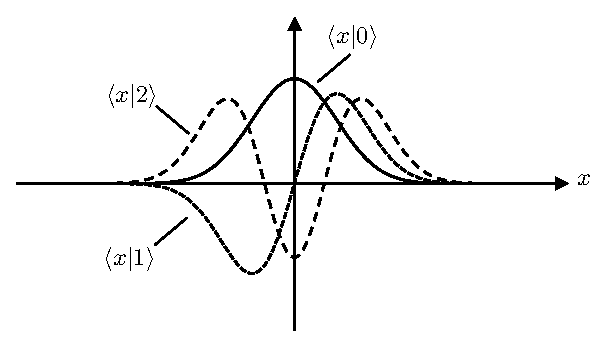
\includegraphics[width=9cm]{fig/3-2_Hermite_Gaussian.eps} 
  \caption{Position representation of the first three energy eigenstates: $\braket{x|0}, \braket {x|1}, \braket {x|2}$.}
  \label{fig:classical_phase_space}
\end{figure}


\subsubsection{Momentum representation of energy eigenstates}

\begin{equation}
  \begin{aligned}
  	\braket{p|n} = \frac{1}{\sqrt{n!}}\braket{p|(\hat a^\dagger)^n|0}
  \end{aligned}
\end{equation}
In the $p$ representation, $\hat x$ is given by
\begin{equation}
  \hat x = \frac i 2 \frac {\partial}{\partial p}.
\end{equation}
such that $[\hat x, \hat p] = i/2$ is satisfied. Therefore, 
\begin{equation}
  \hat a = \hat x + i\hat p = \frac i 2 \frac{\partial}{\partial p} + ip = i\left( p+\frac{1}{2}\frac{\partial}{\partial p} \right),
  \label{eq:annihilation_in_p}
\end{equation}
\begin{equation}
  \hat a^\dagger = \hat x - i\hat p = \frac i 2 \frac{\partial}{\partial p} - ip = -i \left(p - \frac{1}{2}\frac{\partial}{\partial p} \right).
  \label{eq:creation_in_p}
\end{equation}
From Eq. (\ref{eq:braket_x_0}) and Eq. (\ref{eq:tranform_position_momentum}),
\begin{equation}
  \braket{p|0} = \int\braket{p|x}\braket{x|0}dx = \frac {(\pi/2)^{1/4}} {\sqrt \pi} 
  \int e^{-x^2}e^{-2ipx}dx = (\pi/2)^{1/4}e^{-p^2}.
\end{equation}
From Eq. (\ref{eq:annihilation_in_x}), (\ref{eq:annihilation_in_p}), (\ref{eq:creation_in_x}), and (\ref{eq:creation_in_p}), we can see the similarity of $x$ representation and $p$ representation; $\hat a$ $\hat a^\dagger$ have $i$ and $-i$ terms, respectively.
Therefore, we can find $\braket{p|1}, \braket{p|2}, \cdots$ as follows:
\begin{equation}
  \braket{p|1} = -i(2/\pi)^{1/4}2pe^{-p^2},
\end{equation}
\begin{equation}
  \braket{p|2} = -2^{-1/2}(2/\pi)^{1/4}(4p^2-1)e^{-p^2},
\end{equation}
In this way, the energy eigenstates $\ket n$ in $x$ and $p$ representations are almost similar; the latter has $(-i)^n$ times difference. The reason behind this will be explained in later chapters.

\begin{comment}
	
\subsubsection{Energy representation of position eigenstates}
Since $\braket{x|n}$ can be derived as shown above, position eigenstate can be given by
\begin{equation}
  \braket {E|x} = \sum_{n=0}^{\infty} \braket{E|n}\braket{n|x} \sum_{n=0}^{\infty} \delta(E-\hbar \omega (n + 1/2))\braket{n|x} 
\end{equation}
We don't see any consequence of this expression at the moment but this reminds you that any quantum state can be expressed by any basis.
\end{comment}


\section{Measurement of observables}
Quantum mechanics uses Hermitian operators to express physical quantities called observables, such as number of photons, electric field, and so on. The expectation value of the observable can be calculated by specifying both the Hermitian operator of the observable and the quantum state. Here we explain how we calculate the observables.
 
\subsection{Expectation value}
Here we show that the expectation value of the observable $\hat A$ with a quantum state $\ket \psi$ is given by
\begin{equation}
  \braket{\hat A} \equiv \braket{\psi|\hat A|\psi}
\end{equation}

In Eq. (\ref{eq:diagonalization_of_Hermitian_operator}), we saw that Hermitian operator can be diagonalized with a unitary operator $\hat U$. In the $x$ representation, $\hat U$ can be represented by $U(x,x')$, which consists of the orthonormal eigenvector of $\hat A$ for various $x'$ with a eigenvalue of $\lambda(x)$. Therefore
\begin{equation}
  \int A(x,x'')U(x'', x')dx'' = \lambda(x')U(x,x').
\end{equation}

First, we express $\ket \psi$ by a linear combination of the eigenvector, i.e.,
\begin{equation}
  \ket \psi = \hat U \ket \phi,
\end{equation}
where $\ket \phi$ shows the weight of eigenvector. Then we multiply $\hat A$ to obtain
\begin{equation}
  \hat A \ket \psi = \hat A \hat U \ket \phi
\end{equation}
Since $\hat A = \hat U\hat D\hat U^\dagger$,
\begin{equation}
  \hat A \ket \psi = \hat U\hat D \ket \phi
\end{equation}

\begin{equation}
  \braket{\psi|\hat A | \psi} = \bra \phi \hat U^\dagger \hat U \hat D \ket \phi = \braket {\phi|\hat D|\phi}
\end{equation}
The meaning of RHS can be clearer by describing in $x$-representation:
\begin{equation}
    \braket{\psi|\hat A | \psi}= \int \phi^*(x)\lambda(x)\phi(x)dx = \int \lambda(x)|\phi(x)|^2 dx
\end{equation}
The RHS is the weighted average of $\lambda(x)$ with a weight of $|\phi(x)|^2$.

In this way, when we evaluate some observable, we express $\psi$ as a linear combination of eigenstates of the observable. Then we calculate the weighted sum of eigenvalue. Such calculation is embedded in $\braket{\psi|\hat A|\psi}$.

In the same manner, we can calculate the expectation of the variance as follows:
\begin{equation}
  \begin{aligned}
  	\braket{(\hat A - \braket{\hat A})^2} &= \braket{\hat A^2 - 2\hat A\braket{\hat A} + \braket{\hat A}^2}\\
  	&= \braket {\hat A^2} - 2\braket{\hat A}\braket{\hat A} + \braket {\hat A}^2\\
  	&= \braket {\hat A^2} - \braket {\hat A}^2\\
  	&= \braket{\psi|\hat A^2|\psi} - \braket{\psi|\hat A|\psi}^2
  \end{aligned}
\end{equation}

\subsection{Commutation relation and simultaneous measurement}

Here we show that, when two Hermitian operators $\hat A$ and $\hat B$ are commutative, i.e., $\hat A \hat B = \hat B \hat A$, there exists a quantum state that is an eigenstate $\ket \phi$ of $\hat A$ and $\hat B$. To prove this, we assume that $\ket {\phi_A}$ is an eigenstate of $\hat A$ with an eigenvalue of $a_0$, i.e., 
\begin{equation}
  \hat A\ket {\phi_0} = a_0 \ket{\phi_0}.
  \label{eq:commutation_A}
\end{equation}
Then let's calculate $\hat A\hat B \ket {\phi_0}$ as
\begin{equation}
  \hat A \hat B \ket{\phi_0} = \hat B \hat A \ket{\phi_0} = a_0 \hat B \ket{\phi_0}.
\end{equation}
This follows that $\hat B \phi_0$ is also an eigenvector of $\hat A$ with an eigenvalue of $a_0$. Therefore, $\hat B\ket{\phi_0}$ is proportional to $\ket \phi_A$, i.e.,
\begin{equation}
  \hat B \ket{\phi_0} = b_0 \ket{\phi_0}
  \label{eq:commutation_B}
\end{equation}
Eq. (\ref{eq:commutation_A}) and Eq. (\ref{eq:commutation_B}) show that $\ket {\phi_0}$ is an eigenvector of $\hat A$ and $\hat B$. This means that we can measure the observables $\hat A$ and $\hat B$ simultaneously. 

On the other hand, if $\hat A$ and $\hat B$ are not commutative, i.e., $\hat A \hat B \neq \hat B \hat A$, the observables $\hat A$ and $\hat B$ cannot be measured simultaneously. $\hat x$ and $\hat p$ are representative examples of such observables. This leads to the uncertainty relation described below.

\subsection{Uncertainty principle}
Uncertainty principle states that, for observables $\hat A$, $\hat B$ with $[\hat A, \hat B] \neq 0$,
\begin{equation}
  \braket {\Delta \hat A^2}\braket{\Delta \hat B^2} \geq \left| \frac{1}{2} \braket {[\hat A, \hat B]}\right|^2,
  \label{eq:uncertainty}
\end{equation}
where
\begin{equation}
\begin{aligned}
  \braket{\hat A} \equiv \braket{\phi|\hat A|\phi}, \Delta \hat A = \hat A - \braket {\hat A},\\
  \braket{\hat B} \equiv \braket{\phi|\hat B|\phi}, \Delta \hat B = \hat B - \braket {\hat B}.
\end{aligned}
\end{equation}

This means that when $[\hat A, \hat B] \neq 0$, it is not possible to reduce the noise or fluctuation of the both observables to zero. 

Eq. (\ref{eq:uncertainty}) can be derived as follows. First, we introduce $\hat C = i[\Delta \hat A, \Delta \hat B]$. We can show that $\hat C$ is Hermitian because
\begin{equation}
\begin{aligned}
  \hat C^\dagger &= -i(\Delta \hat B^\dagger \Delta \hat A^\dagger - \Delta \hat A^\dagger \Delta \hat B^\dagger) \\ 
  &= -i(\Delta \hat B \Delta \hat A - \Delta \hat A \Delta \hat B) = i[\Delta \hat A, \Delta \hat B] = \hat C.
\end{aligned}
\end{equation}
Here we introduce $\hat D = \Delta A + i\lambda \Delta B$, where $\lambda$ is a real number, and calculate $\braket{\hat D^\dagger \hat D} \equiv \braket{\phi | \hat D^\dagger \hat D| \phi}$ for an arbitrary quantum state $\ket \phi$. 
\begin{equation}
  \begin{aligned}
  	\braket{\hat D^\dagger \hat D} &= \braket{(\Delta \hat A - i\lambda\Delta \hat B)(\Delta \hat A + i\lambda\Delta \hat B)} \\
  	&= \braket{\Delta \hat A}^2  + i\lambda\braket{[\Delta \hat A\Delta \hat B - \Delta \hat B \Delta \hat A]} + \lambda^2 \braket{\Delta \hat B}^2\\
  	&= \braket{\Delta \hat A}^2  + \lambda\braket{\hat C} + \lambda^2 \braket{\Delta \hat B}^2\\
  \end{aligned}
\end{equation}
Since $\braket{\phi|\hat D^\dagger\hat D|\phi} = \|\hat D\ket \phi \|^2\geq 0$, the discriminant of the above equation should satisfy
\begin{equation}
  \braket{\hat C}^2 - 4\braket{\Delta \hat A^2}\braket{\Delta \hat B^2} \leq 0.
\end{equation}
This leads to Eq. (\ref{eq:uncertainty}).

\section{Multimode quantum states}
So far, we have considered wavefunctions and quantum states of a one-dimensional harmonic oscillator at a single frequency. In later chapters, we consider light field as a collection of many harmonics oscillators that constitutes many spatial modes, time-frequency modes, and polarizations. Here we explain how to deal with quantum states of multi-mode harmonic oscillators.

The wavefunction of two-mode wavefunction can be denoted as $\psi(x_a, x_b)$, where $x_a$, $x_b$ are the position of two modes denoted by $a$ and $b$, respectively. $|\psi(x_a,x_b)|^2$ gives the probability density that the position of mode $a$ and that of mode $b$ are $x_a$ and $x_b$, respectively. If $\psi(x_a, x_b)$ can be expressed by a product of two functions as
\begin{equation}
  \psi(x_a, x_b) = \psi_a(x_a)\psi_b(x_b),
  \label{eq:separable_wavefunction}
\end{equation}
we regard that $\psi(x_a)$ is \textbf{separable}\index{separable}. If $\psi(x_a, x_b)$ cannot be expressed in such a way, we regards that the two modes are \textbf{entangled}\index{entangled}.

In the bra-ket notation, separable quantum state is denoted as
\begin{equation}
  \ket \psi = \ket {\psi_a}_a \otimes \ket{\psi_b}_b,
\end{equation}
where $\otimes$ denotes tensor product. For example, if we assume that $\ket {\psi_a}_a$ and $\ket{\psi_b}_b$ are M- and N-dimensional vectors, respectively, i.e., $\ket {\psi_a} = (c_{a1}, c_{a2}, \cdots, c_{aM})^T$ and $\ket {\psi_b} = (c_{b1}, c_{b2}, \cdots, c_{bN})^T$,
\begin{equation}
  \ket{\psi_a}_a \otimes \ket{\psi_b}_b = \left(
  \begin{array}{cccc}
  c_{a1}c_{b1} & c_{a1}c_{b2} & \ldots & c_{a1}c_{bN}\\
  c_{a2}c_{b1} & c_{a2}c_{b2} & \ldots & c_{a2}c_{bN}\\
  \vdots & \vdots & \ddots & \vdots \\
  c_{aM}c_{b1} & c_{aM}c_{b2} & \ldots & c_{am}c_{bN}
  \end{array}
  \right),
  \label{eq:separable_quantum_state}
\end{equation}
which constitutes $M \times N$-dimensional vector space. We can see the similarity in Eq. (\ref{eq:separable_wavefunction}) and Eq. (\ref{eq:separable_quantum_state}).

Even if $\ket \psi$ is not separable, we can expand it by energy eigenstates $\ket n$ in the two modes as
\begin{equation}
  \ket \psi = \sum_{m=0}^{\infty}\sum_{n=0}^{\infty}\ket m_a \otimes \ket n_b (\ _a\bra m  \otimes \ _b\bra n)\ket \psi. 
\end{equation}
That is, any quantum state can be expressed by the linear combination of $\ket m_a \otimes \ket n_b$, and the weight is given by the inner product between $\ket m_a \otimes \ket n_b$ and $\ket \psi$.

The above discussion applies to higher dimensions. For N-dimensional harmonic oscillator, the wavefunction is given by $\psi(x_1, x_2, \cdots, x_N)$. We can discuss the separability in the same way as the above. 

\section{Summary}
We have reviewed the basics of quantum harmonic oscillators including the Schr\"odinger equation, wavefunction, energy eigenstates, operators and measurement. Important concepts are summarized below:
\begin{itemize}
	\item Wavefunction $\psi(x)$ is the position representation of quantum state, and $|\psi(x)|^2$ gives the probability density of being at $x$.
	\item From the Schr\"odinger equation of a harmonic oscillator, we can derive energy eigenstate $\ket n$ with an energy $E_n = \hbar \omega (n + 1/2)$.
	\item The representation (position, momentum, and energy) of quantum state is interchangeable by taking the inner product with corresponding eigenstates.
	\item Expectation value of observable of a Hermitian operator $\hat A$ is given by $\braket{\psi|A|\psi}$.
\end{itemize}
